%% 
%% This is file, `info_merkzettel_wichtig.tex',
%% generated with the extract package.
%% 
%% Generated on :  2022/12/06,9:27
%% From source  :  info_merkzettel.tex
%% Using options:  active,generate=info_merkzettel_wichtig,extract-env=mzImportant,copydocumentclass=false,
%% 
    \documentclass[uniLeipzig]{merkzettel}
  

\begin{document}

\begin{mzImportant}
  \mzGraphic{
    \begin{tblr}{
      cells = {c},
      cell{1}{1} = {c=2}{},
      cell{2}{3} = {r=2}{r},
      cell{4}{3} = {r=2}{r},
      cell{6}{3} = {r=2}{r},
      cell{8}{3} = {r=2}{r},
      cell{10}{3} = {r},
      cell{11}{3} = {r=2}{r},
      cell{13}{3} = {r=2}{r},
      cell{15}{3} = {r=3}{r},
      vline{2} = {2-17}{},
      hline{1-2,18} = {-}{},
        }
      \textbf{Äquivalente Formeln $\boldsymbol{\Leftrightarrow}$}               &                                                 & Bezeichnung \\
      $A \land B$                                & $B \land A$                                     & \index{Logische Kommutativität}Kommutativ  \\
      $A \lor B$                                 & $B \lor A$                                      &             \\
      $A \land (B \land C)$                      & $(A \land B) \land C$                           & \index{Logische Assoziativität}Assoziativ  \\
      $A \lor (B \lor C)$                        & $(A \lor B) \lor C$                             &             \\
      $A \land (B \lor C)$                       & $(A \land B) \lor (A \land C)$                  & \index{Logische Distributivität}Distributiv \\
      $A \lor (B \land C)$                       & $(A \lor B) \land (A \lor C)$                   &             \\
      $A \land A$                                & $A$                                             & \index{Idempotenz}Idempotenz  \\
      $A \lor A$                                 & $A$                                             &             \\
      $\neg \neg A$                              & $A$                                             & \index{Involution}Involution  \\
      $\neg (A \land B)$                         & $\neg A \boldsymbol{\lor} \neg B$  & \index{\textsc{De-Morgan}}\textsc{De-Morgan}   \\
      $\neg (A \lor B)$                          & $\neg A \boldsymbol{\land} \neg B$ &             \\
      $A \land (\mathbf{A} \lor B)$ & $A$                                             & \index{Absoption}Absorption  \\
      $A \lor (\mathbf{A} \land B)$ & $A$                                             &             \\
      $A \Rightarrow B$                          & $\mathbf{\neg A} \lor B$           & \index{Elimination}Elimination \\
      $\neg (A \Rightarrow B)$                   & $A \land \neg B$                                &             \\
      $A \Leftrightarrow B$                      & $(A \Rightarrow B) \land (B \Rightarrow A)$     &
    \end{tblr}
  }
\end{mzImportant}

\begin{mzImportant}
  \begin{itemize}
    \item $\bigcup_{i \in \emptyset} M_i = \boldsymbol{\emptyset}$ (,,hinzufügen``)

    \item $\bigcap_{i \in \emptyset} M_i = \boldsymbol{U}$ (,,wegnehmen``)
  \end{itemize}
\end{mzImportant}

\begin{mzImportant}
  \begin{description}
    \item [Injektiv]
          \index{Injektiv}
          $\forall x_1, x_2 \in X:$ \\
          $x_1 \boldsymbol{\neq} x_2 \Leftrightarrow f(x_1) \boldsymbol{\neq} f(x_2)$

    \item [Surjektiv]
          \index{Surjektiv}
          $\forall y \in Y \exists x \in X: \mathbf{y = f(x)}$

    \item [Bijektiv/Invertierbar]
          \index{Bijektiv}
          wenn injektiv und surjektiv
  \end{description}
\end{mzImportant}

\begin{mzImportant}
  \begin{description}
    \item [$\boldsymbol{\equiv}$ Reflexiv]
          \index{Reflexivität}
          $\forall x \in M: (\mathbf{x}, \mathbf{x}) \in R$ \\
          $\Leftrightarrow \text{id}_M \subseteq R$
          % \\ $\not\Leftrightarrow \text{Irreflexiv} \land M \neq \emptyset$

    \item [Irreflexiv]
          \index{Irreflexivität}
          $\forall x \in M: (x, x) \boldsymbol{\notin} R$ \\
          $\Leftrightarrow \text{id}_M \cap R = \emptyset$

    \item [$\boldsymbol{\equiv}$ Sym.]
          \index{Symmetrie}
          $\forall (x,\mathbf{y}) \in R: (\mathbf{y}, x) \in R$ \\
          $\Leftrightarrow R \subseteq R^{-1}$

    \item [$\boldsymbol{\preceq}$ Antis.]
          \index{Antisymmetrie}
          $\forall x,y: ((x,y) \in R \land (y,x) \in R) \Rightarrow \mathbf{x = y}$ \\
          $\Leftrightarrow R \cap R' \subseteq \text{id}_M$

    \item [$\boldsymbol{\equiv}$ Transitiv]
          \index{Transitivität}
          $\forall \mathbf{x},y,\mathbf{z}: ((x,y) \in R \land (y,z) \in R) \Rightarrow (\mathbf{x},\mathbf{z}) \in R$ \\
          $\Leftrightarrow R;R \subseteq R$

    \item [Vollst.]
          \index{Vollständigkeit}
          $\forall \mathbf{x},\mathbf{y} \in M: (x,y) \in R \lor (y,x) \in R$ \\
          $\Leftrightarrow R \cup R^{-1} = M \times M$
  \end{description}
\end{mzImportant}

\begin{mzImportant}
  \begin{description}
    \item [Inverse Relation $R^{-1}$]
          \index{Inverse Relation}
          mit $R \in M \times N :=$ \\
          $\{ (n, m) \in N \times M \mid (m, n) \in R \}$

    \item [Komposition $R ; R$]
          \index{Komposition}
          mit $R' \in N \times P :=$ \\
          $\{ (m, p) \in M \times P \mid \exists n \in N: (m, n) \in R \land (n, p) \in R' \}$

    \item [Leere Relation $\emptyset$]
          \index{Leere Relation}

    \item [Identität $\text{id}_M$]
          \index{Relationsidentität}
          $:= \{ (m,m) \mid m \in M \}$ ($=$)

    \item [Allrelation $M \times M$]
          \index{Allrelation}

    \item [Äquivalenzrelation $\boldsymbol{\equiv}$]
          \index{Äquivalenzrelation}
          reflexiv, symmetrisch und transitiv. (Gleichheit***)

          \item[Äquivalenzklasse $\mathbf{[m]_\equiv}$]
          \index{Äquivalenzklasse}
          auf $M$, Vertreter $m \in M$.

          \begin{align*}
            [m]_\equiv & := \{ x \in M \mid m \equiv x \}        \\
                       & \Leftrightarrow [m]_\equiv = [x]_\equiv
          \end{align*}

    \item [Zerlegung $\boldsymbol{\mathcal{N}}$]
          \index{Zerlegung}
          $\subseteq \mathcal{P}(M)$ von $M$.

          \begin{itemize}
            \item $\emptyset \notin \mathcal{N}$
            \item $M = \bigcup \mathcal{N}$
            \item $N \cap N' = \emptyset$ \\
                  ($N, N' \in \mathcal{N}: N \neq N'$)
            \item (Korrespondiert zur ÄR.)
          \end{itemize}

    \item [Quotient $\mathbf{(M / \equiv)}$]
          \index{Mengenquotient}
          Sei $\equiv$ ÄR. auf $M$. (ist Zerlegung)

          $$(M / \equiv) := \{ [m]_\equiv \mid m \in M \}$$

          \begin{itemize}
            \item (Korrespondiert zur ÄK.)
          \end{itemize}

    \item [Ordnungsrelation $\boldsymbol{\preceq}$]
          \index{Ordnungsrelation}
          reflexiv, antisymmetrisch, transitiv

          \begin{description}
            \item [Minimale $x$] $\forall m \in M \setminus \{ x \}: m \not\preceq x$
                  \index{Minimale Elemente}
                  \index{Maximale Elemente}

            \item [Untere Schranken $m \in \downarrow X$] $\forall x \in X: m \preceq x$
                  \index{Untere Schranken}
                  \index{Obere Schranken}

            \item [Kleinstes] $\min_\preceq X \in X$
                  \index{Kleinstes Element}
                  \index{Größtes Element}
          \end{description}

    \item [Totale Ordnung] $+$ vollständig (Trichotomie)
          \index{Totale Ordnung}
  \end{description}
\end{mzImportant}

\begin{mzImportant}
  \begin{itemize}
    \item $\sqrt[n]{\mathbf{a * b}} = \sqrt[n]{\mathbf{a}} \mathbin{\boldsymbol{*}} \sqrt[n]{\mathbf{b}}$

    \item $\sqrt[\mathbf{n}]{ \sqrt[\mathbf{m}]{a} } = \sqrt[\mathbf{n * m}]{a}$

    \item $\sqrt[n]{a} < \sqrt[n]{b} \quad 0 \leq a < b$

    \item $\sqrt[n+1]{a} < \sqrt[n]{a} \quad 1 < a$

    \item $\sqrt[n]{a} < \sqrt[n+1]{b} \quad 0 < a < 1$
  \end{itemize}

  $$\sqrt[n]{a^n} = |a| \quad a \in \mathbb{R}$$
\end{mzImportant}

\begin{mzImportant}
  \begin{itemize}
    \item $a^{\mathbf{x}} * b^{\mathbf{x}} = (a \mathbf{*} b)^{\mathbf{x}}$

    \item $a^x * a^y = a^{x \boldsymbol{+} y}$

    \item $(a^x)^y = a^{x \boldsymbol{*} y}$

          % \item $a^x < a^y \quad 1 < a, x < y$
          % \item $a^x > a^y \quad 0 < a < 1, x < y$
          % \item $a^x < b^x \quad a < b, 0 < x$
          % \item $a^x > b^x \quad a < b, x < 0$
  \end{itemize}
\end{mzImportant}

\begin{mzImportant}
  $$x = \sum_{n = 0}^\infty \frac{a_n}{10^n}$$
\end{mzImportant}

\begin{mzImportant}
  \begin{description}
    \item [Minimum]
          \index{Minimum in $\mathbb{R}$}
          $\min(A) := a_0$ \\
          $\Leftrightarrow \forall a \in A: \mathbf{a_0} \boldsymbol{\leq} a$

    \item [Maximum]
          \index{Maximum in $\mathbb{R}$}
          $\max(A) := a_0$ \\
          $\Leftrightarrow \forall a \in A: \mathbf{a} \boldsymbol{\leq} a_0$
  \end{description}
\end{mzImportant}

\begin{mzImportant}
  \begin{description}
    \item [Infimum (klein)] $\inf(A)$ \\
          \index{Infimum}
          $:= \mathbf{\max} \{ s \in \mathbb{R} \mid \forall a \in A: \mathbf{s} \boldsymbol{\leq} a \}$

    \item [Supremum (gro\ss)] $\sup(A)$ \\
          \index{Supremum}
          $:= \mathbf{\min} \{ s \in \mathbb{R} \mid \forall a \in A: \mathbf{a} \boldsymbol{\leq} s \}$
  \end{description}
\end{mzImportant}

\begin{mzImportant}
  $$\sum^n i = \frac{n * (n + 1)}{2}$$
\end{mzImportant}

\begin{mzImportant}

  \paragraph{Geom. Summe} $q \in \mathbb{R} \setminus \{ 0 \}, n \in \mathbb{N}_0$
  \index{Geometrische Summe}

  $$\sum_{i=0}^n q^i = \frac{1 - q^{n+1}}{1 - q}$$

  \paragraph{\textsc{Bernoulli} Unglei.} $n \in \mathbb{N}_0, x \geq -1$
  \index{\textsc{Bernoulli} Ungleichung}

  $$(1 + x)^n \geq 1 + nx$$

  \paragraph{Binom. Koeff.} $\binom{n}{k} = \frac{n!}{k! (n - k)!}$
  \index{Binomial Koeffizient}
\end{mzImportant}

\begin{mzImportant}
  $$(a + b)^n = \sum_{k=0}^n \binom{n}{k} * a^{n - k} b^k$$
\end{mzImportant}

\begin{mzImportant}
  \begin{description}
    \item [Lemma] $|x * y| = |x| * |y|$

    \item [Dreiecksungleichung]
          \index{Dreiecksungleichung}
          $|x + y| \boldsymbol{\leq} |x| + |y|$

    \item [Umgekehrte \linebreak Dreiecksungleichung]
          \index{Umgekehrte Dreiecksungleichung}
          $\linebreak ||x| - |y|| \leq |x - y|$
  \end{description}
\end{mzImportant}

\begin{mzImportant}
  \begin{gather*}
    a_n \xrightarrow{n \rightarrow \infty} a \Leftrightarrow \\
    \forall \epsilon > 0 \exists n_0 \in \mathbb{N} \forall n \in \mathbb{N} n \geq n_0: \\
    \mathbf{|a_n - a| \leq \epsilon} \\
    (a - \epsilon \leq a_n \leq a + \epsilon)
  \end{gather*}
\end{mzImportant}

\begin{mzImportant}
  Beschränkt + monoton $\Rightarrow$ konvergent:

  $$\lim_{n \rightarrow \infty} a_n = \begin{cases}
      \boldsymbol{\inf} \{ a_n \mid n \in \mathbb{N} \} \quad (a_n)_\text{\emph{fall.}} \\
      \boldsymbol{\sup} \{ a_n \mid n \in \mathbb{N} \} \quad (a_n)_\text{\emph{steig.}}
    \end{cases}$$
\end{mzImportant}

\begin{mzImportant}
  \begin{gather*}
    a_n \xrightarrow{n \rightarrow \infty} \boldsymbol{\infty} \Leftrightarrow \\ \forall R \boldsymbol{>} 0 \exists n \geq n_0 \in \mathbb{N}: a_n \boldsymbol{\geq} R \\
    a_n \xrightarrow{n \rightarrow \infty} \boldsymbol{-\infty} \Leftrightarrow \\ \forall R \boldsymbol{<} 0 \exists n \geq n_0 \in \mathbb{N}: a_n \boldsymbol{\leq} R
  \end{gather*}
\end{mzImportant}

\begin{mzImportant}
  \begin{itemize}
    \item Konvergent $\Rightarrow$ beschränkt

    \item Unbeschränkt $\Rightarrow$ divergent
  \end{itemize}
\end{mzImportant}

\begin{mzImportant}
  \begin{gather*}
    \lim_{n \rightarrow \infty} a_n = \lim_{n \rightarrow \infty} b_n = a \\
    \forall n \geq N \in \mathbb{N}: \mathbf{a_n \leq c_n \leq b_n} \\
    (\exists) \lim_{n \rightarrow \infty} c_n = \mathbf{a}
  \end{gather*}
\end{mzImportant}

\begin{mzImportant}
  $$\lim_{n \rightarrow \infty} a_n = a \Rightarrow \lim_{n \rightarrow \infty} {a_n}_k = a$$

  (da $n_k$ mnt. steigend)

  $$\forall (a_n)_{n \in \mathbb{N}} \exists {({a_n}_k)_{k \in \mathbb{N}}}_\text{\emph{mnt.}}$$

  (nicht streng!)
\end{mzImportant}

\begin{mzImportant}
  $${(a_n)_{n \in \mathbb{N}}}_{\text{\emph{beschr.}}} \Rightarrow \exists h_\text{\emph{Häuf.}}$$

  (Beschränkte Teilfolgen besitzen mind. einen Häufungspunkt)
\end{mzImportant}

\begin{mzImportant}
  \begin{gather*}
    \forall \epsilon > 0 \exists n_0 \in \mathbb{N} \forall n, m \geq n_0:\\
    |a_n - a_m| \leq \epsilon
  \end{gather*}
\end{mzImportant}

\begin{mzImportant}
  \begin{description}
    \item[Geom.]
      \index{Geometrische Reihe}
      $\sum_{k=0}^\infty q^k = \frac{1}{1- q} \quad q \in (-1;1)$

    \item [Harmon.]
          \index{Geometrische Reihe}
          $\sum_{k=1}^\infty \frac{1}{k}$ divergent

    \item [Allg. Harmon.]
          \index{Allgemeine Harmonische Reihe}
          $\sum_{k=1}^\infty \frac{1}{k^\alpha}$ konvergiert $\forall \mathbf{\alpha > 1}$
  \end{description}
\end{mzImportant}

\begin{mzImportant}
  \begin{description}
    \item [\textsc{Cauchy}]
          \index{\textsc{Cauchy}-Kriterium}
          \begin{align*}
            \Leftrightarrow & {(\sum_{k=1}^n a_k)_{n \in \mathbb{N}}} \text{\emph{\textsc{ Cauchy}}} \\
                            & (\sum_{k=1}^\infty a_k)_\text{konv.}                                   \\
            \Leftrightarrow & \forall \epsilon > 0 \exists n_0 \in \mathbb{N} \forall n > m > n_0 :  \\
                            & | \sum_{k=m + 1}^n a_k | \leq \epsilon
          \end{align*}

    \item [Notwendig]
          \begin{align*}
            (\sum_{n=1}^\infty a_n)_\text{konv.} \Rightarrow \lim_{n \rightarrow \infty} a_n = \boldsymbol{0} \\
            \lim_{n \rightarrow \infty} a_n \neq 0 \Rightarrow (\sum_{n=1}^\infty a_n)_\text{div.}
          \end{align*}

    \item [Beschränkt]
          $a_n \geq 0$ ($\Rightarrow$ \emph{mnt.}) $\forall n \in \mathbb{N}$
          $$(\sum_{n=1}^\infty a_n)_\text{\emph{beschr.}} \Leftrightarrow (\sum_{n=1}^\infty a_n)_\text{konv.}$$

    \item [Majorante]
          \index{Majorantenkriterium}
          $0 \leq \mathbf{a_n \leq b_k} \quad \forall n \in \mathbb{N}$\\
          % (Min. $\leq$ Major.)
          \index{Majorante}
          \index{Minorante}
          $$(\sum_{n=1}^\infty b_n)_\text{konv.} \Leftrightarrow (\sum_{n=1}^\infty a_n)_\text{konv.}$$

    \item [Quotient]
          \index{Quotientenkriterium}
          $a_n \geq 0 \quad \forall n \in \mathbb{N}$
          $$
            \lim_{n \rightarrow \infty} \frac{a_{n + 1}}{a_n} \begin{cases}
              \mathbf{< 1} \rightarrow (\sum_{n = 1}^\infty a_n)_\text{konv.} \\
              \mathbf{> 1} \rightarrow (\sum_{n = 1}^\infty a_n)_\text{div.}
            \end{cases}
          $$

    \item [Wurzel]
          \index{Wurzelkriterium}
          $a_n \geq 0 \quad \forall n \in \mathbb{N}$
          $$
            \lim_{n \rightarrow \infty} \sqrt[n]{a_n} \begin{cases}
              \mathbf{< 1} \rightarrow (\sum_{n = 1}^\infty a_n)_\text{konv.} \\
              \mathbf{> 1} \rightarrow (\sum_{n = 1}^\infty a_n)_\text{div.}
            \end{cases}
          $$

    \item [Absolut]
          \index{Absolute Konvergent}
          $$(\sum_{n=1}^\infty | a_n |)_\text{konv.} \Rightarrow (\sum_{n=1}^\infty a_n)_\text{konv.}$$

          $$| \sum_{n=1}^\infty a_n | \leq \sum_{n=1}^\infty | a_n |$$

          (Dreiecksungleichung)
          \index{Reihendreiecksungleichung}

    \item [Leibniz] $(a_n)_{n \in \mathbb{N}}$ mnt. Nullfolge
          \index{Leibniz-Kriterium}
          $$(\sum_{n=1}^\infty (-1)^n * a_n)_\text{konv.}$$

    \item [Grenzwert] $a_n, b_n \geq 0 \quad \forall n \in \mathbb{N}$
          \index{Grenzwertkriterium}
          \begin{gather*}
            \lim_{n \rightarrow \infty} \frac{a_n}{b_n} \mathbf{> 0} \Rightarrow \\
            (\sum_{n=1}^\infty a_n)_\text{konv.} \Leftrightarrow (\sum_{n=1}^\infty b_n)_\text{konv.}
          \end{gather*}
  \end{description}
\end{mzImportant}

\begin{mzImportant}
  $$\exp(x) := \sum_{n = 0}^\infty \frac{x^n}{x!}$$
\end{mzImportant}

\begin{mzImportant}
  $$\exp(x) * \exp(y) = \exp(x + y)$$
\end{mzImportant}

\begin{mzImportant}
  $$(\sum_{n = 0}^\infty a_n)(\sum_{n = 0}^\infty b_n) = \sum_{n = 0}^\infty \sum_{k = 0}^n a_k b_{n - k}$$
\end{mzImportant}

\begin{mzImportant}
  \index{Gro\ss-O-Notation}
  \paragraph{Gro\ss-O-Notation}
  Kosten $C_f(n)$ mit $g: \mathbb{N} \rightarrow \mathbb{R} \exists c > 0 \exists n_0 > 0 \forall n \geq n_0$

  \begin{description}
    \item [Untere Schranke] $\boldsymbol{\Omega} (f)$ \\
          \index{Untere Schranke Komplexität}
          $C_f(n) \boldsymbol{\geq} c * g(n)$

    \item [Obere Schranke] $\boldsymbol{O}(f)$ \\
          \index{Obere Schranke Komplexität}
          $C_f(n) \boldsymbol{\leq} c * g(n)$

    \item [Exakte Schranke] $\boldsymbol{\Theta} (f)$ \\
          \index{Exakte Schranke Komplexität}
          $C_f(n) \in \Omega (f) \cap O(f)$ \\
          Polynom $k$ten Grades $\in \Theta (n^k)$
  \end{description}

  (Beweis: $g$ und $c$ finden)
\end{mzImportant}

\begin{mzImportant}
  \begin{description}
    \item [Elementare Operationen, Kontrollstr.]
          $\mathbf{\in O(1)}$

    \item [Schleifen]
          $\in$ $i$ Wiederholungen $\boldsymbol{*}$ $O(f)$ teuerste Operation

    \item [Abfolge]
          $O(g)$ nach $O(f)$ $\in O(\boldsymbol{\max} (f;g))$

    \item [Rekursion]
          $\in$ $k$ Aufrufe $\boldsymbol{*}$ $O(f)$ teuerste Operation
  \end{description}
\end{mzImportant}

\begin{mzImportant}
  \index{Mastertheorem}
  \paragraph{Mastertheorem} $a \geq 1$, $b > 1$, $\Theta \geq 0$

  \begin{gather*}
    T(n) = a * T( \frac{n}{b} ) + \Theta (n^k) \\
    \Rightarrow \begin{cases}
      \Theta ( n^k ) \quad          & a < b^k \\
      \Theta ( n^k \log n ) \quad   & a = b^k \\
      \Theta ( n^{\log_b a} ) \quad & a > b^k
    \end{cases}
  \end{gather*}
\end{mzImportant}

\begin{mzImportant}
  \paragraph{Skip}
  \index{Skip-Liste}

  \mzGraphic{
    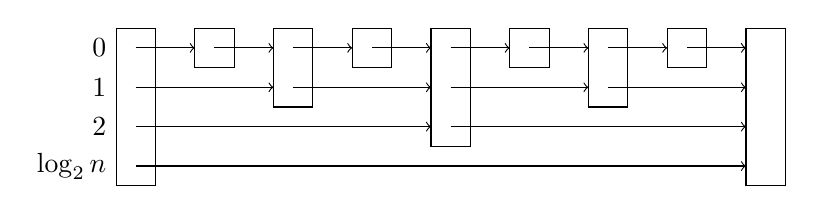
\begin{tikzpicture}[scale=.5,yscale=-1]
      \draw
      (-2,0) rectangle (-1,4)

      (0,0) rectangle (1,1)
      (2,0) rectangle (3,2)
      (4,0) rectangle (5,1)
      (6,0) rectangle (7,3)
      (8,0) rectangle (9,1)

      (10,0) rectangle (11,2)
      (12,0) rectangle (13,1)

      (14,0) rectangle (15,4);

      \draw[->] (-1.5,.5) -- (0,.5);
      \draw[->] (0.5,.5) -- (2,.5);
      \draw[->] (2.5,.5) -- (4,.5);
      \draw[->] (4.5,.5) -- (6,.5);
      \draw[->] (6.5,.5) -- (8,.5);

      \draw[->] (8.5,.5) -- (10,.5);
      \draw[->] (10.5,.5) -- (12,.5);
      \draw[->] (12.5,.5) -- (14,.5);

      \draw[->] (-1.5,1.5) -- (2,1.5);
      \draw[->] (2.5,1.5) -- (6,1.5);
      \draw[->] (6.5,1.5) -- (10,1.5);
      \draw[->] (10.5,1.5) -- (14,1.5);

      \draw[->] (-1.5,2.5) -- (6,2.5);
      \draw[->] (6.5,2.5) -- (14,2.5);

      \draw[->] (-1.5,3.5) -- (14,3.5);

      \draw
      (-2,.5) node[left] {$0$}
      (-2,1.5) node[left] {$1$}
      (-2,2.5) node[left] {$2$}
      (-2,3.5) node[left] {$\floor{\log_2 n}$};
    \end{tikzpicture}
  }

  \begin{itemize}
    \item Zeiger auf Ebene $i$ zeigt zu nächstem $2^i$ Element
    \item Suchen $\in O(\log n)$
  \end{itemize}

  \begin{description}
    \item [(Perfekt)]
          \index{Perfekte Skip-Liste}
          Einfügen, Löschen $\mathbf{\in O(n)}$ (Vollst. Reorga.)

    \item [Randomisiert]
          \index{Randomisierte Skip-Liste}
          Höhe zufällig (keine vollst. Reorga.) \\
          $P(h) = \frac{1}{2^{h + 1}}$: Einfügen, Löschen $\mathbf{\in O(\log n)}$
  \end{description}
\end{mzImportant}

\begin{mzImportant}
  \paragraph{Sortierproblem}
  \index{Sortierproblem}

  \begin{description}
    \item[Gegeben] (endliche) Folge von Schlüsseln (von Daten) $(K_i)_{i \in I}$
    \item[Gesucht] Bijektive Abbildung $\pi: I \rightarrow I$ (Permutation), sodass $K_{\pi(i)} \leq K_{\pi(i + 1)} \quad \forall i \in I$
  \end{description}
\end{mzImportant}

\begin{mzImportant}
  \begin{description}
    \item [Ordnung] \emph{Allgemein} vs. \emph{speziell}: Ordnung wird nur über Schlüsselvergleiche hergestellt
          \index{Allgemeine Suche}
          \index{Spezielle Suche}
    \item [Relation] \emph{Stabil} vs. \emph{instabil}: Vorherig relative Reihenfolge bleibt erhalten
          \index{Stabile Suche}
          \index{Instabile Suche}
    \item [Speicher] \emph{In situ} vs. \emph{ex situ}: Zusätzlicher Speicher notwendig
          \index{In situ Suche}
          \index{Ex situ Suche}
    \item [Lokal] \emph{Intern} vs. \emph{extern}: Alles im RAM oder Mischung vorsortierter externer Teilfolgen
          \index{Interne Suche}
          \index{Externe Suche}
  \end{description}
\end{mzImportant}

\begin{mzImportant}
  \begin{description}
    \item [Anzahl der Inversionen]
          \index{Anzahl der Inversionen}
          Anzahl kleinerer Nachfolger für jedes Element:
          \begin{gather*}
            \text{inv} (L) := |\{ (i,j) \mid \\
            0 \leq i < j \leq n - 1, \\
            L[i] \geq L[j] \}|
          \end{gather*}

    \item [Anzahl der Runs]
          \index{Run}
          Ein \emph{Run} ist eine sortierte Teilliste, die nicht nach links oder rechts verlängert werden kann.
          Die Anzahl der Runs ist:
          \begin{gather*}
            \text{runs} (L) := |\{ i \mid \\
            0 \leq i < n - 1, \\
            L[i + 1] < L[i]  \}| \mathbf{+ 1}
          \end{gather*}

    \item [Längster Run]
          \index{Längster Run}
          Anzahl der Elemente der längsten sortierten Teilliste:
          \begin{gather*}
            \text{las} (L) := \max \{ r.\text{len} \mid \\
            r \text{ ist Run in } L \} \\
            \text{rem} (L) := L.\text{len} - \text{las} (L)
          \end{gather*}
  \end{description}
\end{mzImportant}

\begin{mzImportant}
  Jedes allgemeine Sortierverfahren benötigt im Worst- und Average-case Schlüsselvergleiche von mindestens:

  $$\Omega (n \log n)$$
\end{mzImportant}

\begin{mzImportant}
  \paragraph{Lexikographische Ordnung $\mathbf{\leq}$}
  \index{Lexikographische Ordnung}
  Sei $A = \{ a_1, \dots, a_n \}$ ein Alphabet, dass sich mit gegebener Ordnung $a_1 < \cdots < a_n$ wie folgt auf dem Lexikon $A* = \bigcup_{n \in \mathbb{N}_0} A^n$ fortsetzt:
  \begin{align*}
                    & v = (v_1, \dots, v_p) \leq w = (w_1, \dots, w_q)   \\
    \Leftrightarrow & \forall 1 \leq i \leq p: v_i = w_i \quad p \leq q  \\
    \lor            & \forall 1 \leq j \leq i: v_j = w_j \quad v_i < w_i
  \end{align*}

  \paragraph{Fachverteilen}
  \index{Fachverteilen}
  Sortieren von $n$ $k$-Tupeln in $k$ Schritten: Sortieren nach letztem Element, vorletzem usw.
\end{mzImportant}

\begin{mzImportant}
  % TODO: Merge Shell sort cells and add this text:
  % Abhängig von Sprunggrö\ss en $h_i$: $O(n \log n)$, $O(n^\frac{3}{2})$ bis $O(n^2)$ (h_i = 1)
  \mzGraphic{
    \begin{tblr}{
      row{2} = {c},
      row{12} = {c},
      cell{1}{1} = {r=2}{},
      cell{1}{2} = {r=2}{c},
      cell{1}{3} = {r=2}{c},
      cell{1}{4} = {c=3}{c},
      cell{1}{7} = {c=3}{c},
      cell{1}{10} = {r=2}{r},
      cell{3}{2} = {c},
      cell{3}{3} = {c},
      cell{3}{4} = {c},
      cell{3}{5} = {c},
      cell{3}{6} = {c},
      cell{3}{7} = {c},
      cell{3}{8} = {c},
      cell{3}{9} = {c},
      cell{3}{10} = {r=3}{c},
      cell{4}{2} = {c},
      cell{4}{3} = {c},
      cell{4}{4} = {c},
      cell{4}{5} = {c},
      cell{4}{6} = {c},
      cell{4}{7} = {c},
      cell{4}{8} = {c},
      cell{4}{9} = {c},
      cell{5}{2} = {c},
      cell{5}{3} = {c},
      cell{5}{4} = {c},
      cell{5}{5} = {c},
      cell{5}{6} = {c},
      cell{5}{7} = {c},
      cell{5}{8} = {c},
      cell{5}{9} = {c},
      cell{6}{4} = {c=2}{c},
      cell{6}{6} = {c=2}{c},
      cell{6}{8} = {c=2}{c},
      cell{7}{2} = {c},
      cell{7}{3} = {c},
      cell{7}{4} = {c=2}{c},
      cell{7}{6} = {c=2}{c},
      cell{7}{8} = {c=2}{c},
      cell{7}{10} = {r=5}{c},
      cell{8}{2} = {c},
      cell{8}{3} = {c},
      cell{8}{4} = {c=2}{c},
      cell{8}{6} = {c=2}{c},
      cell{8}{8} = {c=2}{c},
      cell{9}{2} = {c},
      cell{9}{3} = {c},
      cell{9}{4} = {c=2}{c},
      cell{9}{6} = {c=2}{c},
      cell{9}{8} = {c=2}{c},
      cell{10}{2} = {c},
      cell{10}{3} = {c},
      cell{10}{4} = {c=2}{c},
      cell{10}{6} = {c=2}{c},
      cell{10}{8} = {c=2}{c},
      cell{11}{2} = {c},
      cell{11}{3} = {c},
      cell{11}{4} = {c=2}{c},
      cell{11}{6} = {c=2}{c},
      cell{11}{8} = {c=2}{c},
      cell{12}{1} = {c=10}{},
      cell{13}{2} = {c},
      cell{13}{3} = {c},
      cell{13}{4} = {c=2}{c},
      cell{13}{6} = {c=2}{c},
      cell{13}{8} = {c=2}{c},
      cell{13}{10} = {r},
      hline{1,3,6-7,12-14} = {-}{},
        }
      \textbf{Algo.} & \textbf{Stabil} & \textbf{Mem.} & \textbf{Schlüsselvergleiche} &  &  & \textbf{Satzbewegungen} &  &  & \\

      &  &  & $C_B$ & $C_A$ & $C_W$ & $M_B$ & $M_A$ & $M_W$ & \\

      Selection & \ding{55} & $1$ & $\frac{n (n - 1)}{2}$ & $\frac{n (n - 1)}{2}$ & $\frac{n (n - 1)}{2}$ & $3 (n - 1)$ & $3 (n - 1)$ & $3 (n -1)$ & \begin{sideways}$O(n^2)$\end{sideways}\\

      Insertion & \ding{51} & $1$ & $n - 1$ & $\overset{n \rightarrow \infty}{\approx} \frac{n (n - 1)}{4} + n - \ln n$ & $\frac{n (n - 1)}{2}$ & $2 (n - 1)$ & $\frac{n^2 + 3n - 4}{4} + n - 1$ & $\frac{n^2 + 3n - 4}{2}$ & \\

      Bubble & \ding{51} & $1$ & $\frac{n (n - 1)}{2}$ & $\frac{n (n - 1)}{2}$ & $\frac{n (n - 1)}{2}$ & $0$ & $\frac{3n (n - 1)}{4}$ & $\frac{3n (n - 1)}{2}$ & \\

      &  &  & \textbf{Best-case} &  & \textbf{Average-case} &  & \textbf{Worst-case} &  & \\

      Shell & \ding{55} & $1$ & - &  & - &  & - &  & \begin{sideways}$O(n \log n)$\end{sideways}\\

      Quick & \ding{55} & $\log n$ & $n \log n$ & & $n \log n$ & & $n^2$ & & \\

      Turnier & \ding{55} & $2n - 1$ & $n \log n$ & & $n \log n$ & & $n \log n$ & & \\

      Heap & \ding{55} & $1$ & $n \log n$ & & $n \log n$ &  & $n \log n$ &  & \\

      Merge & \ding{51} & $n$ & $n \log n$ &  & $n \log n$ &  & $n \log n$ &  & \\

      \textbf{Untere Schranke $\Omega (n \log n)$ für allgemeine Sortierverfahren} & & & & & & & & & \\

      Distribution & \ding{51} & $n$ & $n$ &  & $n$ &  & $n \log n$, $n^2$ &  & $O(n)$
    \end{tblr}
  }
\end{mzImportant}

\begin{mzImportant}
  \begin{description}
    \item [Einfach] keine Schleife
          \mzInline{
            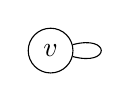
\begin{tikzpicture}[every loop/.style={}]
              \node [circle,draw] {$v$} edge[loop right] ();
            \end{tikzpicture}
          }
          oder Doppelkanten
          \mzInline{
            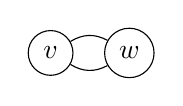
\begin{tikzpicture}
              \node (v) [circle,draw] {$v$};
              \node (w) at (1,0) [circle,draw] {$w$};
              \path (v) edge [bend left] (w);
              \path (w) edge [bend left] (v);
            \end{tikzpicture}
          }
          \index{Einfacher Graph}

    \item [Zusammenhängend]
          \index{Zusammenhängender Graph}
          Für jede zwei Knoten gibt es genau eine Folge von Kanten die sie verbindet

    \item [Azyklisch]
          \index{Azyklischer Graph}
          kein Zyklus (Cycle)
          \mzInline{
            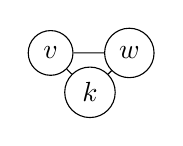
\begin{tikzpicture}
              \node (v) [circle,draw] {$v$};
              \node (w) at (1,0) [circle,draw] {$w$};
              \node (k) at (.5,-.5) [circle,draw] {$k$};

              \draw (v) -- (w) -- (k) -- (v);
            \end{tikzpicture}
          }
  \end{description}
\end{mzImportant}

\begin{mzImportant}
  \begin{description}
    \item[Ordnung] Max. Anzahl von Kindern jedes Knoten eines Baums
      \index{Baumordnung}

    \item[Tiefe] Anzahl Kanten zwischen einem Knoten und Wurzel
      \index{Knotentiefe}

    \item[Stufe] Alle Knoten gleicher Tiefe
      \index{Baumstufe}

    \item[Höhe] Max. Tiefe $+ 1$
      \index{Baumhöhe}
  \end{description}
\end{mzImportant}

\begin{mzImportant}
  \begin{description}
    \item[Geordnet] Kinder erfüllen Ordnung von links nach rechts
      \index{Geordneter Baum}

    \item[Vollständig]
      \index{Vollständiger Baum}
      Alle Blätter auf gleicher Stufe, jede Stufe hat max. Anzahl von Kindern
  \end{description}
\end{mzImportant}

\begin{mzImportant}
  \begin{description}
    \item[Strikt]
      \index{Strikter Binärbaum}
      Jeder Knoten hat $0$ oder $2$ Kinder (Kein Knoten hat genau $1$ Kind).

    \item[Vollständig]
      \index{Vollständiger Binärbaum}
      Jeder Knoten au\ss er der letzten Stufe hat genau $2$ Kinder.

    \item[Fast Vollständig]
      \index{Fast Vollständiger Binärbaum}
      Vollständig, au\ss er Blätter können rechts fehlen.

    \item[Ausgeglichen]
      \index{Ausgeglichener Binärbaum}
      Vollständig, aber Blätter auf letzten $2$ Stufen
  \end{description}
\end{mzImportant}

\begin{mzImportant}
  $$(AB)_{ij} = \sum_{k=1}^m a_{ik}b_{kj}$$

  (Reihe $\times$ Spalte)
\end{mzImportant}

\end{document}
